\chapter{Vacuum Energy, Unification, and Grassmann Superspace}

These notes follow Leonard Susskind's sixth lecture in the supplementary course on supersymmetry and grand unification, with curation by LazyingArt LLC. We begin exactly where the lecture begins: not with a formal definition of superspace, but with a student question about the Casimir effect. From that concrete entry point the argument unfolds in a deliberate chain. First we ask what vacuum energy means and what would count as honest evidence for it. Then we clarify what a supersymmetry generator actually does. Only after that do we ask why low-energy supersymmetry is worth taking seriously, why cosmology sharpens the whole question of energy, and finally what kind of Grassmann calculus is needed if supersymmetric theories are to be written in a controlled way.

\section{Vacuum Energy, Casimir Effect, and Honest Evidence}

Susskind reenters the subject by answering unfinished business from the previous lecture. What is the Casimir effect? Take two reflecting plates a distance \(L\) apart. In empty space there are vacuum processes. One may picture them as virtual particle pairs, or as zero-point oscillators associated with the quantum fields. In the lecture those are presented as two descriptions of the same thing. Once the plates are introduced, the vacuum fluctuations are modified by the boundary conditions. Virtual loops that would have occupied the region freely are interrupted, reflected, and reorganized by the plates.

The result is that the vacuum energy depends on the plate separation. That is the first mathematical point, and it is all we need. If the energy is a function of \(L\), then we may read it as a potential energy, and a force follows:
\begin{equation}
F(L)=-\frac{dE_{\mathrm{Casimir}}(L)}{dL}.
\end{equation}
This is the lecture's real use of the Casimir effect. It is not a place to derive a famous formula. Susskind even hesitates over the exact power law, and we should not pretend the lecture settled it. What matters here is the mechanism: altered vacuum energy means a force between the plates.

For the electromagnetic vacuum that force is ordinarily attractive. Susskind adds, with a characteristic caution, that a fermionic loop would likely reverse the sign. The details are not the point. The point is that the force is generated because the vacuum energy changes when the plates are moved.

But the lecture then immediately becomes more severe about interpretation. The Casimir force is measurable, but it is a very small effect, and one may still think of it as a force between nearby plates without insisting that it is the cleanest possible evidence for the gravitating energy of empty space. The stronger question is: what do we really mean by energy? Energy gravitates. Mass gravitates. If the vacuum really carries energy, then the honest evidence should be gravitational.

That is the pivot of the section. The lecture moves from laboratory boundary conditions to cosmology. The real evidence for vacuum energy, Susskind says, is the accelerated expansion of the universe. The Casimir effect is suggestive. Cosmic acceleration is the direct gravitational evidence.

\subsection{Question \& Answer}

\paragraph{Question.} What is actually mysterious about vacuum energy?

\paragraph{Answer.} Not its existence. This distinction is one of the lecture's central clarifications. Quantum field theory predicts zero-point energy for every field. In that sense vacuum energy is not an unknown substance waiting to be discovered; it is a structural consequence of the theory. The mystery is that the observed vacuum energy is so tiny.

The lecture is especially good on the psychology of this. For a long time physicists convinced themselves that vacuum energy must vanish exactly, because it appeared to be absent to very high precision and because naive quantum-field-theoretic estimates were so much larger. Then better observations showed that vacuum energy was not absent after all. The resulting surprise was real, but the real surprise was never that empty space could carry energy. It was that the amount of energy that gravitates is so extraordinarily small.

That distinction will matter again when we return to cosmology. We are not looking for a reason why vacuum energy exists at all. We are looking at a world in which it exists, gravitates, and yet is remarkably suppressed.

\section{What a Supersymmetry Generator Really Does}

The next question comes from a possible misunderstanding about many-particle states. If bosons can pile into the same state, what happens when supersymmetry acts? Do we create a whole population of fermions in that state? The lecture slows down here, and it is worth following that slowdown.

The supersymmetry transformation is generated by an operator \(Q\). Susskind compares it with an ordinary symmetry generator, such as angular momentum, but only to emphasize the difference. A rotation generator makes an infinitesimal rotation, and repeated action can be compounded into a finite one. A supersymmetry generator is not like that. It is fermionic, and its action is local in fermion number:
\begin{equation}
Q\,|B\rangle \propto |F\rangle,
\qquad
Q\,|F\rangle \propto |B\rangle,
\qquad
Q^2=0.
\end{equation}
The lecture's verbal formulation is even more concrete: \(Q\) does not turn a system of bosons into a system of fermions. It removes one boson and replaces it by one fermion, or vice versa. On a many-body state it changes the occupation only by one unit. That is why Susskind says that supersymmetry changes us by one unit of fermion number.

The nilpotency \(Q^2=0\) is the algebraic reason this does not build up into a macroscopic conversion. One act of \(Q\) changes a boson into a fermion. Act again with the same fermionic generator and the result vanishes. The lecture is careful to linger over this because it clears away a conceptual obstacle before any discussion of motivation.

\subsection{Question \& Answer}

\paragraph{Question.} Why can repeated action of \(Q\) not turn a Bose population into a Fermi population?

\paragraph{Answer.} Because \(Q\) is not an ordinary bosonic generator that can be compounded over and over again. Its square vanishes:
\begin{equation}
Q^2=0.
\end{equation}
So the action of supersymmetry is not “convert the whole system.” It is “change one boson into one fermion, or one fermion into one boson,” and then stop. The analogy with an infinitesimal rotation is useful only up to the point where it breaks: rotations can be compounded indefinitely, but fermionic generators cannot.

\section{Why Low-Energy Supersymmetry Is Worth Taking Seriously}

Only now does the lecture ask directly what supersymmetry may buy us. The student puts the question bluntly: is there motivation other than cancelling vacuum energy? Susskind's answer is, roughly, yes, a little bit, and then he organizes the rest of the middle lecture around three motivations. He also fixes the scale of the discussion: by supersymmetry he means supersymmetry low enough to matter for experiments not too far beyond present reach, with the LHC very much in mind.

The list is:
\begin{enumerate}
\item control of the Higgs self-energy;
\item stable new particles, especially dark-matter candidates;
\item more precise gauge-coupling unification.
\end{enumerate}
The first two are developed here; the third leads naturally into the next section.

\paragraph{The Higgs self-energy problem.}
The lecture phrases the issue qualitatively, not through a loop integral but through the physical effect of self-energy diagrams. The Higgs mass is shifted by vacuum fluctuations attached to the Higgs line. Left to itself, that shift would naturally drive the Higgs mass to a very high scale. Since the ordinary particle masses are responses to the Higgs phenomenon, everything else would be dragged upward with it.

This is the naturalness problem in the register of the lecture. The dangerous diagrams are not merely large; they threaten to relocate the whole low-energy world. Supersymmetry is attractive because it pairs bosonic and fermionic contributions in such a way that the most dangerous pieces cancel. The lecture does not derive the cancellation quantitatively here, and we should not clutter the argument with formulas it did not motivate. The structural point is enough: if the symmetry survives to low enough energies, the Higgs self-energy is controlled.

\paragraph{Stable superpartners and dark matter.}
The second motivation comes from decay chains. The lecture divides the world into ordinary particles and their superpartners. When a superpartner decays, it decays into an ordinary particle plus another superpartner. Schematically,
\begin{equation}
\tilde X \rightarrow X+\tilde Y \rightarrow X+Y+\tilde Z \rightarrow \cdots
\end{equation}
and the superpartner never disappears from the chain. If one starts with a superpartner, one ends with a superpartner. Therefore the chain terminates at a state of minimum superpartner energy, the lightest superpartner or LSP. In the simple version of the lecture's story, the LSP is stable.

That makes supersymmetry immediately interesting for dark matter. Dark matter is believed to be particulate, long-lived on cosmological time scales, and weakly coupled to ordinary matter. A stable superpartner is exactly that kind of object. Susskind also takes time to explain why the dark particle must be weakly interacting. If it were strongly coupled, electrically charged, or too readily scattered by ordinary matter, it would lose energy and collapse into the visible galactic disk instead of remaining in a diffuse halo. So a viable candidate should be weakly interacting and, very likely, neutral.

The lecture then adds a useful cosmological beat. In the hot early universe thermal equilibrium would populate ordinary particles and superparticles comparably. As the temperature fell, unstable heavy states would decay away. If the LSP is stable, a relic abundance could remain. No relic-density formula is derived here, but the physical logic is exactly the one Susskind wants on the page: supersymmetry naturally provides the sort of particle one needs.

He also keeps the theory modest. The lecture does not claim we know which superpartner is lightest. Depending on the version of the theory, it might be photino-like, Higgsino-like, gravitino-like, or something mixed. The point is not the exact identity; it is the structural existence of a stable endpoint.

\section{Running Couplings and Higher-Precision Unification}

The third motivation arrives through renormalization. Susskind returns to a familiar phenomenon: electric charge is screened. At shorter distances, or equivalently higher energies, the effective electromagnetic coupling is larger. He then introduces the notation \(\alpha\) for the fine-structure constant and observes that it is more convenient to plot \(\alpha^{-1}\), since the inverse coupling runs roughly linearly in the approximation he has in mind. In that language the electromagnetic inverse coupling slopes downward with energy.

The lecture then moves, in this order, to the electroweak coupling and only afterward to the strong coupling. The electroweak inverse coupling also runs roughly linearly, with a different slope, so the two weakly coupled sectors seem to head toward a crossing at high energy. Only then does the strong coupling enter. Because of asymptotic freedom, quantum chromodynamics runs the other way: the strong coupling gets smaller at short distance, so its inverse gets larger.

The lecture's image of this running is not abstract. It is tied directly to Feynman diagrams. A photon exchanged between charged particles may contain an electron-positron loop. At large distances that loop contributes to screening; at short distances there is effectively no room for it. The variation of couplings with scale is thus read physically from the loops that can dress the exchange process. This is why Susskind insists that running couplings are defined by Feynman diagrams.

At the level of the curves, the lecture wants us to remember only the broad pattern:
\begin{equation}
\alpha_{\mathrm{em}}^{-1}(E)\ \text{and}\ \alpha_{\mathrm{ew}}^{-1}(E)\ \text{decrease with }E,
\qquad
\alpha_s^{-1}(E)\ \text{increases with }E.
\end{equation}
If one extrapolates these curves using the plain Standard Model, they show a tempting tendency to meet, but they do not really join. They miss each other by too much.

That is where supersymmetry matters. Once superpartners are added into the brew, new loops appear. The electron loop that affects the photon can be replaced by a loop of the electron's superpartner; analogous modifications occur throughout the other sectors. The slopes change. The lecture's punchline is that with suitably light superpartners the three inverse couplings extrapolate to a common point with unexpectedly good accuracy:
\begin{equation}
\alpha_{\mathrm{em}}^{-1}(E_U)\approx
\alpha_{\mathrm{ew}}^{-1}(E_U)\approx
\alpha_s^{-1}(E_U),
\qquad
E_U\sim 10^{15}\text{--}10^{16}\,\mathrm{GeV}.
\end{equation}
No one has measured physics there. What is measured is the low-energy data, after which the theory is extrapolated upward by calculating the relevant diagrams. But that is precisely why Susskind calls this higher-precision unification: getting two lines to cross is not very impressive, while getting three to meet cleanly at one point is much harder to dismiss as accident.

The lecture then sharpens the phenomenology. This is not exact supersymmetry. The superpartners need not have the same mass as the ordinary particles. But they cannot be too heavy. If they are split far upward, their loops only switch on too late, the three couplings fail to meet, the Higgs self-energy problem reappears, and the dark-matter scale becomes less compelling. Thus the three motivations are tied together by the same rough requirement: if supersymmetry is to do us any good in these domains, it had better set in not too far above experimentally accessible energies.

Two further remarks in the lecture belong here. First, superpartners do not define new interactions. They carry the same gauge quantum numbers as the particles whose partners they are, and precisely for that reason they enter the same loop corrections. Second, Susskind adds a cautious comment about gravity: because gravitational charge is energy, a gravitational coupling would strengthen with energy and its inverse would fall. That suggests a common high scale, though he is careful not to oversell the comparison between gravity and the three gauge forces.

\section{Vacuum Energy in Cosmology and the Friedmann Balance}

From unification the lecture swings, by way of a student question, into a long cosmological detour. The question is not idle. What is the difference between the Higgs divergence and the vacuum-energy divergence? Susskind answers it before he ever writes a cosmological equation, and the order matters.

\subsection{Question \& Answer}

\paragraph{Question.} What is the difference between the Higgs divergence and the vacuum-energy divergence?

\paragraph{Answer.} Vacuum-energy diagrams are just virtual processes in empty space. They contribute to the energy density of the vacuum itself. Higgs self-energy diagrams are different because they are connected to the Higgs line. The presence of the Higgs particle acts, in Susskind's phrase, like an impurity in the vacuum. That impurity modifies the surrounding vacuum fluctuations and thereby shifts the Higgs mass. The two phenomena are related, but one is the energy of empty space and the other is the modification of that vacuum by the presence of a specific particle.

That answer then opens the cosmology detour. What is special about vacuum energy, as opposed to ordinary matter or radiation, is how it behaves as the universe expands.

For ordinary non-relativistic matter the energy density falls because the number of particles in a comoving volume stays fixed while the volume grows. Radiation falls faster still, because the expansion not only dilutes the quanta but stretches their wavelengths and lowers the energy of each one. Vacuum energy does not dilute at all. The lecture states this in words; the clean mathematical summary is
\begin{equation}
\rho_{\mathrm{matter}}\propto a^{-3},
\qquad
\rho_{\mathrm{radiation}}\propto a^{-4},
\qquad
\rho_{\mathrm{vacuum}}=\text{constant}.
\end{equation}
Here \(a(t)\) is the scale factor, which Susskind treats informally as the radius or expansion factor of the universe.

This means that a component that was initially negligible eventually dominates. Radiation dominates first, then matter, and finally vacuum energy. In the lecture's rough contemporary numbers, the universe today is about \(70\%\) vacuum energy and \(30\%\) everything else. One hears the live lecture thinking aloud here: the precise crossover time is not the point; the ordering is.

\begin{figure}[t]
\centering

\includegraphics[width=0.58\textwidth]{lecture_06_figure_03.png}
\caption{Geometry equals energy in the cosmological equation.}
\end{figure}

At the climax of this detour Susskind writes the slogan that organizes the rest of the discussion: geometry equals energy. The first term he isolates on the board is the expansion term
\begin{equation}
\left(\frac{\dot a}{a}\right)^2,
\end{equation}
the first genuinely geometric contribution in the time-time Einstein equation.

The wider board then shows the intended balance. One term comes from the rate of expansion, another from spatial curvature, and the right-hand side is decomposed into matter, radiation, and vacuum energy, with matter itself split into ordinary and dark components. A cautious cleaned-up reconstruction of the board's mathematical content is
\begin{equation}
\left(\frac{\dot a}{a}\right)^2 \pm \frac{1}{a^2}
\sim
\rho_{\mathrm{matter}}+\rho_{\mathrm{radiation}}+\rho_{\mathrm{vacuum}},
\end{equation}
together with
\begin{equation}
\rho_{\mathrm{matter}}=\rho_{\mathrm{ordinary}}+\rho_{\mathrm{dark}}.
\end{equation}

\begin{remark}
The structure of this equation is secure in the lecture and in the selected frames; the overall normalization is not. We therefore keep the Friedmann balance at the level of a careful structural reconstruction. The curvature term is written as \(\pm 1/a^2\) because the sign depends on whether the universe is open, closed, or flat.
\end{remark}

\begin{figure}[t]
\centering

\includegraphics[width=0.88\textwidth]{lecture_06_figure_04.png}
\caption{Friedmann balance of expansion, curvature, and energy content.}
\end{figure}

\begin{figure}[t]
\centering
\begin{tikzpicture}
\draw (-1.7,1.5) rectangle (1.7,-0.3);
\draw (3.1,1.7) rectangle (8.4,-0.5);
\node at (0,1.0) {$\left(\dfrac{\dot a}{a}\right)^2$};
\node at (0,0.2) {$\pm\,\dfrac{1}{a^2}$};
\node at (0,-0.9) {geometry};
\node at (2.4,0.6) {$=$};
\node at (5.75,1.0) {$\rho_{\mathrm{matter}}+\rho_{\mathrm{radiation}}+\rho_{\mathrm{vacuum}}$};
\node at (5.75,0.1) {$\rho_{\mathrm{matter}}=\rho_{\mathrm{ordinary}}+\rho_{\mathrm{dark}}$};
\node at (5.75,-1.1) {energy};
\end{tikzpicture}
\caption{Schematic reconstruction of the board layout: geometry on the left, cosmic contents on the right.}
\end{figure}

This is the point at which the lecture itself pauses and almost asks, how did we get into this? We got into it because a question about vacuum-energy diagrams versus Higgs self-energy forced us to ask what vacuum energy really does in an expanding universe. Once that question is asked, the cosmology is not optional.

\subsection{Question \& Answer}

\paragraph{Question.} How can energy be conserved if vacuum energy density does not dilute as the universe expands?

\paragraph{Answer.} Susskind's answer is deliberately bizarre: in this cosmological setting the total energy is exactly conserved and exactly zero. One must frame that sentence correctly. It is not a blanket statement about every spacetime in general relativity. It is the content of the cosmological Hamiltonian constraint in the setting being discussed.

The lecture first describes the expansion term as a kind of kinetic energy of the expanding universe and says that, in the energy language one is trying to force onto the problem, that contribution is negative. Then it writes the Einstein equation as geometry on the left and energy density on the right. The next move is the decisive one: put everything on one side. The result is no longer merely an equality between two sides of a board calculation. It is a constraint:
\begin{equation}
H_{\mathrm{tot}}=0.
\end{equation}
Schematically,
\begin{equation}
\left(\frac{\dot a}{a}\right)^2
\pm
\frac{1}{a^2}
-
\left(
\rho_{\mathrm{matter}}+\rho_{\mathrm{radiation}}+\rho_{\mathrm{vacuum}}
\right)
=0.
\end{equation}
The lecture interprets the quantity on the left as the canonical Hamiltonian of the cosmological system. So if vacuum energy does not dilute, that does not violate the relevant conservation law. It changes which terms are balancing which. Matter and radiation may decrease, vacuum energy may stay fixed, and the compensating geometric part adjusts so that the total Hamiltonian constraint remains zero. In Susskind's phrase, that is the rule of the game.

\section{Grassmann Numbers, Superspace, and Superfields}

Only after this cosmological excursion does the lecture consciously return to supersymmetry proper. A student asks whether Grassmann numbers actually appear in the Lagrangian. Susskind answers yes, in two different ways.

First, fermion fields themselves are Grassmann-valued. Bosonic fields take ordinary numerical values; fermionic fields anticommute. That is already part of standard field theory. The second appearance is the one he wanted to reach all along: in a supersymmetric theory there are additional coordinates, Grassmann coordinates \(\theta\), and fields may depend on them as well as on the ordinary spacetime coordinates.

The lecture describes this in an exploratory way rather than a heavily formal one. We have the ordinary coordinates \(x^\mu\), but we also have two complex Grassmann coordinates, or equivalently four real ones. These are not large extra dimensions. They are tiny in the sense that they are nilpotent:
\begin{equation}
\theta^2=0.
\end{equation}
That is why Susskind says we cannot move around in them the way we move around in ordinary space. But they are enough to organize the component fields of a supersymmetric multiplet into a single object.

Ordinary fields are functions of \(x\). A superfield is a function of both \(x\) and \(\theta\):
\begin{equation}
\Phi=\Phi(x,\theta).
\end{equation}
Because the \(\theta\)'s square to zero, the theta-expansion terminates after finitely many terms. In the four-real-theta schematic form used in the lecture,
\begin{equation}
\Phi(x,\theta)
=
\phi(x)
+\theta_\alpha\psi_\alpha(x)
+\theta_\alpha\theta_\beta z_{\alpha\beta}(x)
+\cdots
+\theta_1\theta_2\theta_3\theta_4\,D(x).
\end{equation}
This should be read as bookkeeping, not as a finalized convention. The important point is that a superfield packages a finite set of ordinary bosonic and fermionic fields. Terms with an odd number of \(\theta\)'s are Grassmann-valued; terms with an even number are ordinary-number-valued.

Once we accept that fields and Lagrangian densities can depend on \(\theta\), the structure of the action changes as well. We no longer integrate only over spacetime. We integrate over superspace:
\begin{equation}
S=\int d^4x\,d^4\theta\,\mathcal{L}(x,\theta).
\end{equation}
That is where the lecture deliberately stops and asks the next question. What could such an integral possibly mean?

\section{Grassmann Integration as the Calculus of Supersymmetry}

The answer begins from an ordinary formula. Susskind writes a definite integral of a derivative on the board before he says anything about Grassmann variables. That is not accidental. He wants a model.

\begin{figure}[t]
\centering

\includegraphics[width=0.86\textwidth]{lecture_06_figure_05.png}
\caption{Definite integral of a derivative.}
\end{figure}

For an ordinary function \(F(x)\) that dies off at spatial infinity, we have
\begin{equation}
\int_{-\infty}^{\infty}\frac{dF}{dx}\,dx
=
F(\infty)-F(-\infty)
=
0.
\end{equation}
The lecture uses this as the prototype for the Grassmann rule: the definite integral of a derivative should vanish.

The other preliminary point is just as important. Grassmann integration is not an indefinite integral, and it is not a sum of infinitesimal pieces. It is a definite integral over the whole theta-space. In fact, the lecture goes even further: in the one-variable case, the integral turns out to be the same operation as the derivative.

\subsection{Question \& Answer}

\paragraph{Question.} What do we mean by integrating over Grassmann variables?

\paragraph{Answer.} We mean a linear operation, defined so as to mimic the ordinary rule for definite integrals of total derivatives and fixed by a very small number of conventions.

For a single Grassmann variable \(\theta\), the lecture argues as follows:
\begin{enumerate}
\item Demand linearity.
\item Impose the analog of the ordinary total-derivative rule,
\begin{equation}
\int d\theta\,\frac{d}{d\theta}f(\theta)=0.
\end{equation}
\item Choose \(f(\theta)=\theta\). Since \(\dfrac{d}{d\theta}\theta=1\), we obtain
\begin{equation}
\int d\theta\,1=0.
\end{equation}
\item Fix the remaining normalization by convention:
\begin{equation}
\int d\theta\,\theta=1.
\end{equation}
\end{enumerate}
That is already the whole one-variable theory, because every function of one Grassmann variable has the form
\begin{equation}
f(\theta)=a+b\theta.
\end{equation}
Therefore
\begin{equation}
\int d\theta\,f(\theta)=\int d\theta\,(a+b\theta)=b.
\end{equation}
The integral simply extracts the coefficient of the highest theta term. In this one-variable case it is identical to the derivative:
\begin{equation}
\int d\theta\,(a+b\theta)=b=\frac{d}{d\theta}(a+b\theta).
\end{equation}
This is why the lecture says there is no analog of an indefinite integral. One cannot ask for a function whose derivative is \(\theta\), because that function would have to contain \(\theta^2\), and \(\theta^2\) vanishes.

The two-variable case is only slightly richer. Writing the variables as \(\theta\) and \(\bar\theta\), the most general function is
\begin{equation}
f(\theta,\bar\theta)=a+\bar\theta\psi+\bar\psi\,\theta+b\,\bar\theta\theta.
\end{equation}
There are only four terms because \(\theta^2=\bar\theta^2=0\). If we adopt the measure ordering
\begin{equation}
\int d\theta\,d\bar\theta\,\bar\theta\theta=1,
\end{equation}
then every term except the quadratic top component integrates to zero, and we get
\begin{equation}
\int d\theta\,d\bar\theta\,f(\theta,\bar\theta)=b.
\end{equation}

\begin{remark}
The sign depends on ordering, and the lecture corrects itself on this point in real time. With the convention used here,
\[
\int d\bar\theta\,d\theta\,\bar\theta\theta=-1.
\]
Reversing the order of the measure or of the Grassmann variables changes the sign.
\end{remark}

This is where the lecture ends and where the conceptual payoff becomes visible. The rule sounds trivial: integrate over theta and you extract the top component. But that trivial-looking rule is what makes superspace useful. A supersymmetric Lagrangian can be built from superfields and their derivatives, and integrating over the theta's picks out exactly the component that turns into the ordinary action while preserving the boson-fermion structure of the theory. That is why Susskind keeps saying, in effect, that this is the point of it. We are not learning a curiosity. We are assembling the calculus by which supersymmetric theories are actually constructed.

\section{Summary}

The lecture begins with the Casimir effect, but only as a way of asking what vacuum energy really means. From there it sharpens the distinction between the existence of vacuum energy and the mystery of its tiny size, clarifies that a supersymmetry generator changes fermion number one unit at a time and satisfies \(Q^2=0\), lays out three reasons to care about low-energy supersymmetry, detours through cosmology to explain why vacuum energy is special and how the Friedmann equation becomes a zero-Hamiltonian constraint, and finally returns to supersymmetry by introducing superfields and the Berezin calculus. The chapter therefore ends exactly where the lecture ends: with the formal machinery ready, and with the expectation that concrete supersymmetric examples can now be built on top of it.